\usepackage{titlesec}
\newcommand{\subsubsubsection}[1]{\paragraph{#1}\mbox{}\\}
\setcounter{secnumdepth}{4}
\setcounter{tocdepth}{4}
% the above things have to be place here, or all titles will compromise  --Jordan

\section{Experiment}
present here experimental results of the method you have implemented with plots, graphs, images and visualizations.

\subsection{StyleGAN}
In this section we will present result of style fusion of source image \textbf{Fig \ref{fig:source image}} and target image \textbf{Fig \ref{fig:target image}}. The fusion image are present in \textbf{Fig \ref{fig:stylechange}}. According to this result, there are several points that we can discuss. We will divide it into good result and bad result.

\subsubsection{Good result}
As you can see in \textbf{Fig \ref{fig:stylechange}}. The style interpolation of reconstructed source image and reconstructed target image is very successful. We can actually see the hairstyle, faces and background of reconstructed source image gradually fuse into those of reconstructed target image with smoothness. This result proof that interpolation of latent code in latent space actually leads to style fusion of image space.

\subsubsection{Bad result}
According to \textbf{Fig \ref{fig:source image}}, \textbf{Fig \ref{fig:target image}} and \textbf{Fig \ref{fig:stylechange}}, the reconstruction of source image and target image is quite a failure. After some discussion, we find out some points that may lead to this terrible result.

\subsubsubsection {Face position problem}
During implementation, we find that the reconstructed image will change globally if we slightly scale the original image. \textbf{Fig \ref{fig:face position problem}} can fully explain this problem. Both part of image contains original image and reconstructed image. The two images of left part of \textbf{Fig \ref{fig:face position problem}} is the same to \textbf{Fig \ref{fig:source image}} and upper left of \textbf{Fig \ref{fig:stylechange}}. We just cut a little fraction below the neck on the original image, the reconstructed image varies a lot (show in right part of \textbf{Fig \ref{fig:face position problem}}). To be more specific, compared to reconstructed image that do not cut, reconstructed image has more hair, wrinkles. Moreover, the hair, wrinkles have nothing to do with the the neck (cut place). After discussion, we attribute this result to that GAN based model are inherently very hard to control the generated result.

\subsubsubsection {Origin Goal Problem}
The main goal of StyleGAN based model is to use latent code to generate diverse results, while our goal is to use latent code to reconstruct original image, which is totally opposite. This might be a potential reason of our bad result.

\subsubsubsection {Domain gap Problem}
The style encoder is trained on FFHQ dataset, which consists mostly of Caucasian and African. Our source and target image are both Asian, which may lead to a domain gap problem.

\subsubsubsection {Latent code space Problem}
Losing information is inevitable when encoding the high dimensional images to low dimension latent vectors. Due to this, we will lose considerable information when we perform style encoding, leading to that StyleGAN generator can not generate images similar to original images.


\begin{figure}
\centering
    \begin{minipage}[t]{0.48\textwidth}
    \centering
    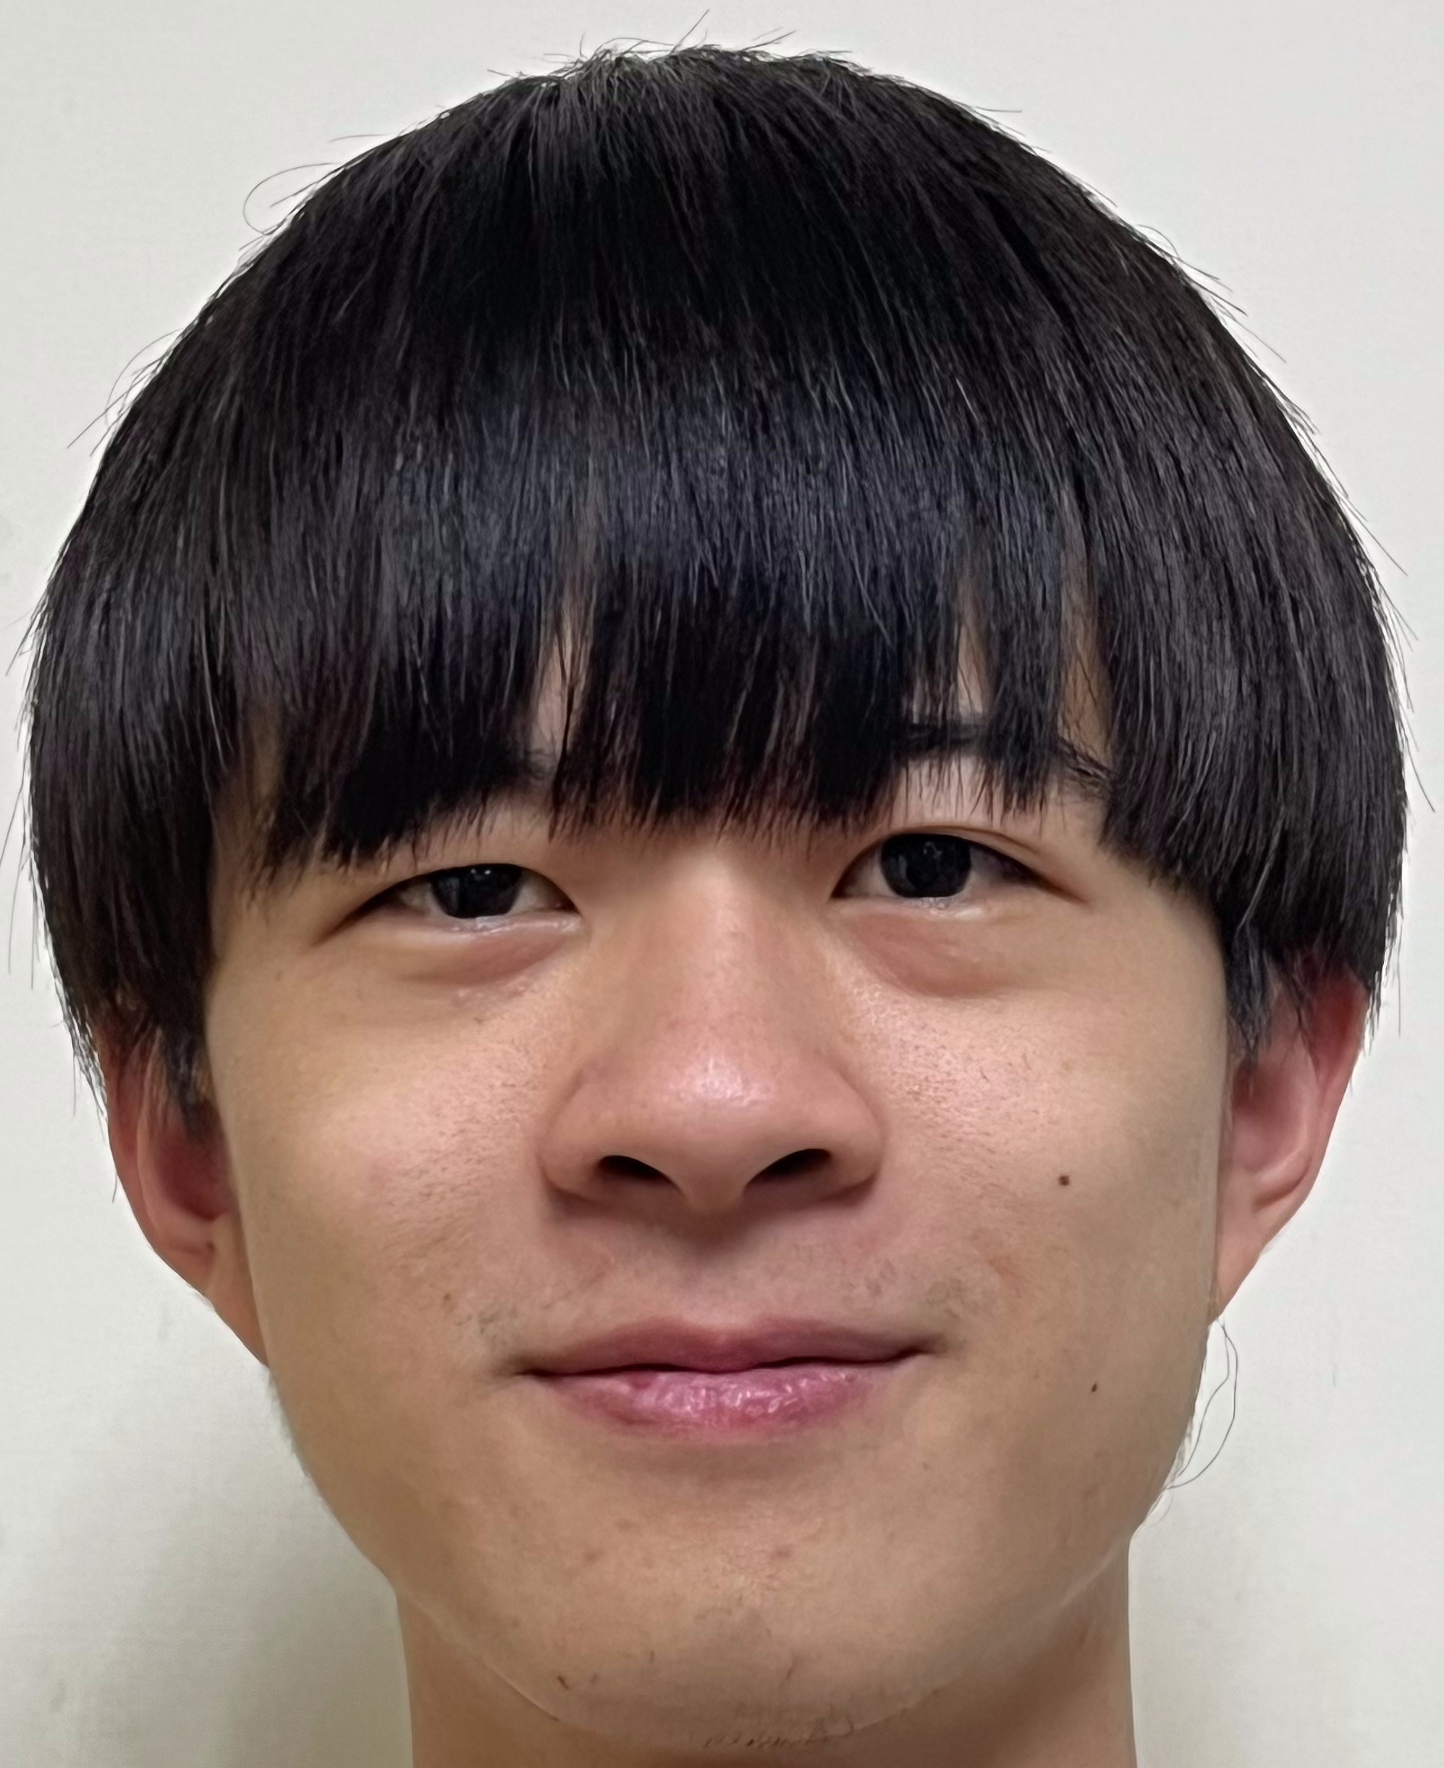
\includegraphics[width=3cm]{fig/source_image.png}
    \caption{source image}
    \label{fig:source image}
    \end{minipage}
    \begin{minipage}[t]{0.48\textwidth}
    \centering
    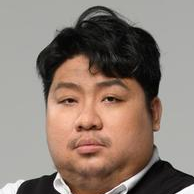
\includegraphics[width=3cm]{fig/target_image.png}
    \caption{target image}
    \label{fig:target image}
    \end{minipage}
\end{figure}

\begin{figure}[ht]
\centering
    \centering
    \includegraphics[scale=.05]{fig/change.png}
    \caption{Style fusion between source image and target image, upper left corner is the original reconstructed source image; while lower right corner is the original reconstructed target image}
    \label{fig:stylechange}
\end{figure}

\begin{figure}
  \centering
  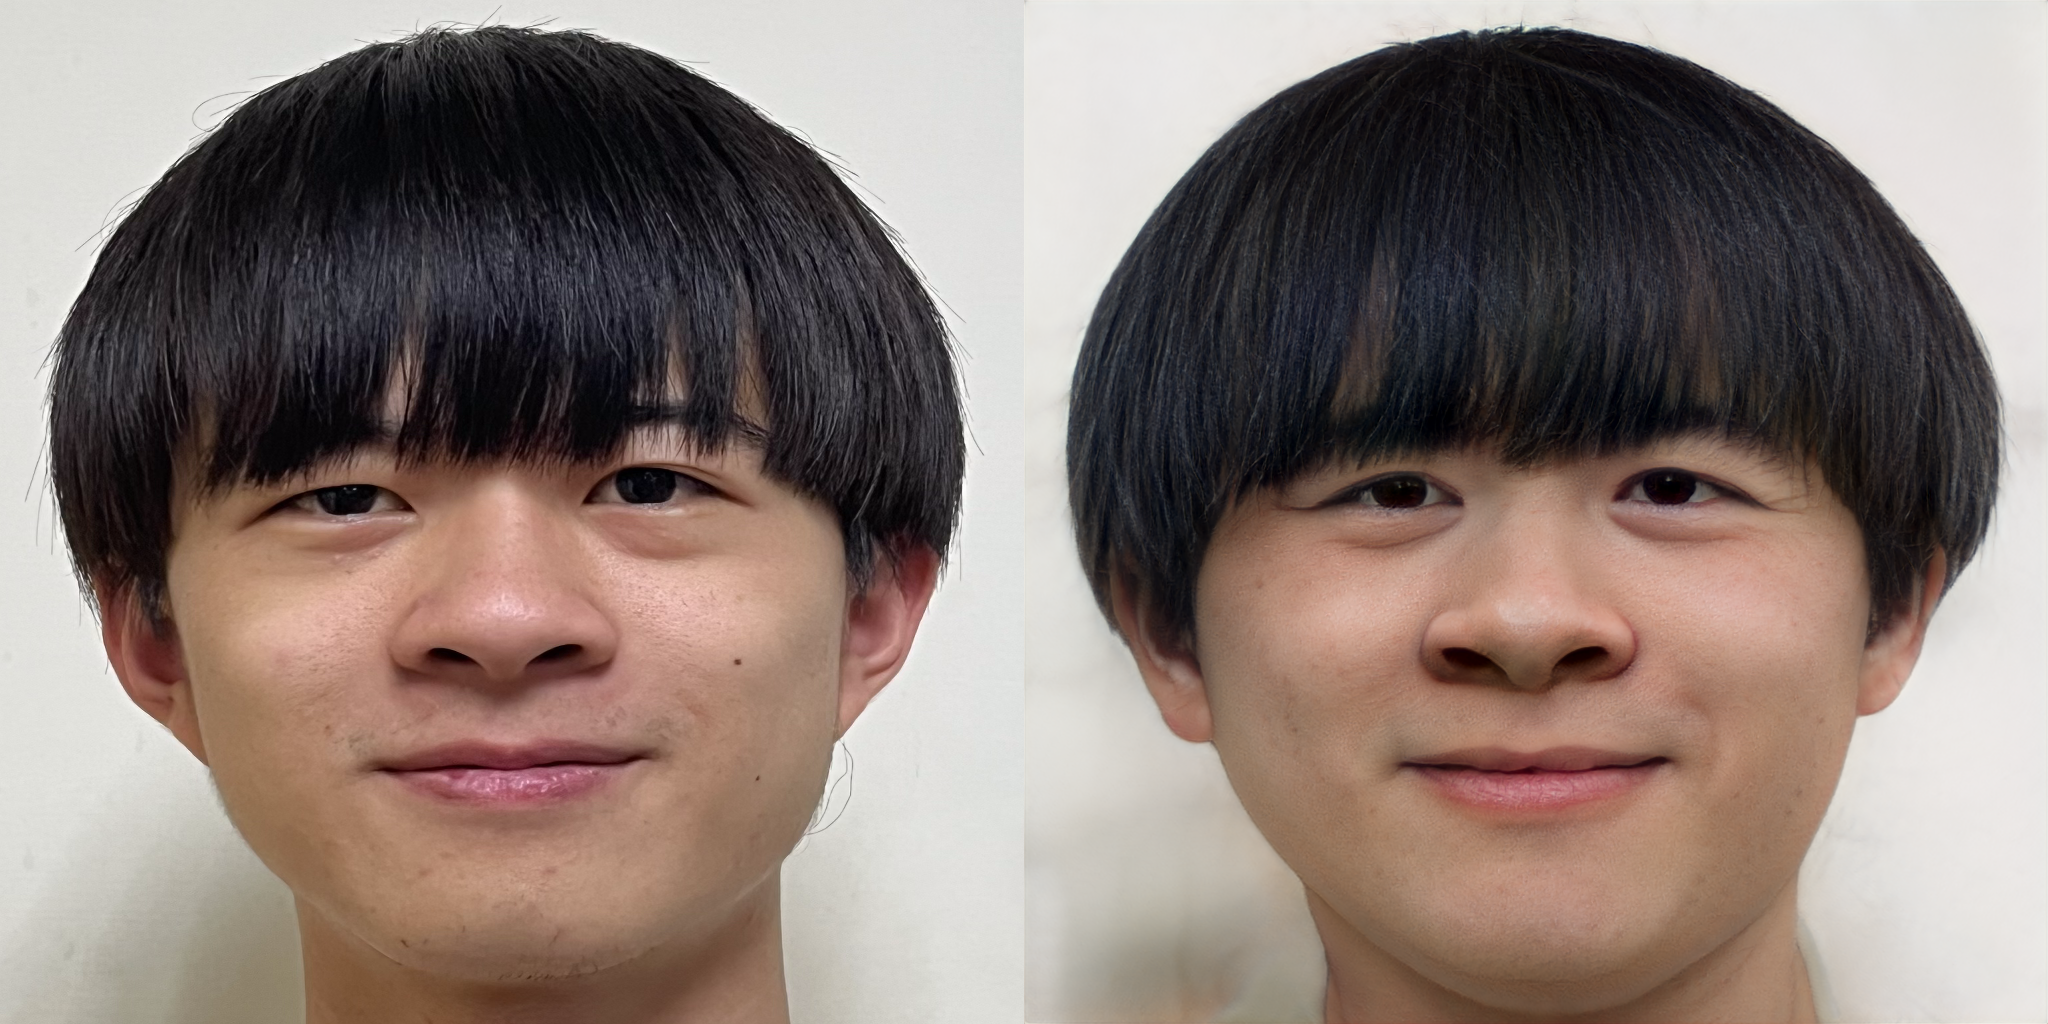
\includegraphics[scale=0.05]{fig/couple_result.png}
  \hspace{1in}
  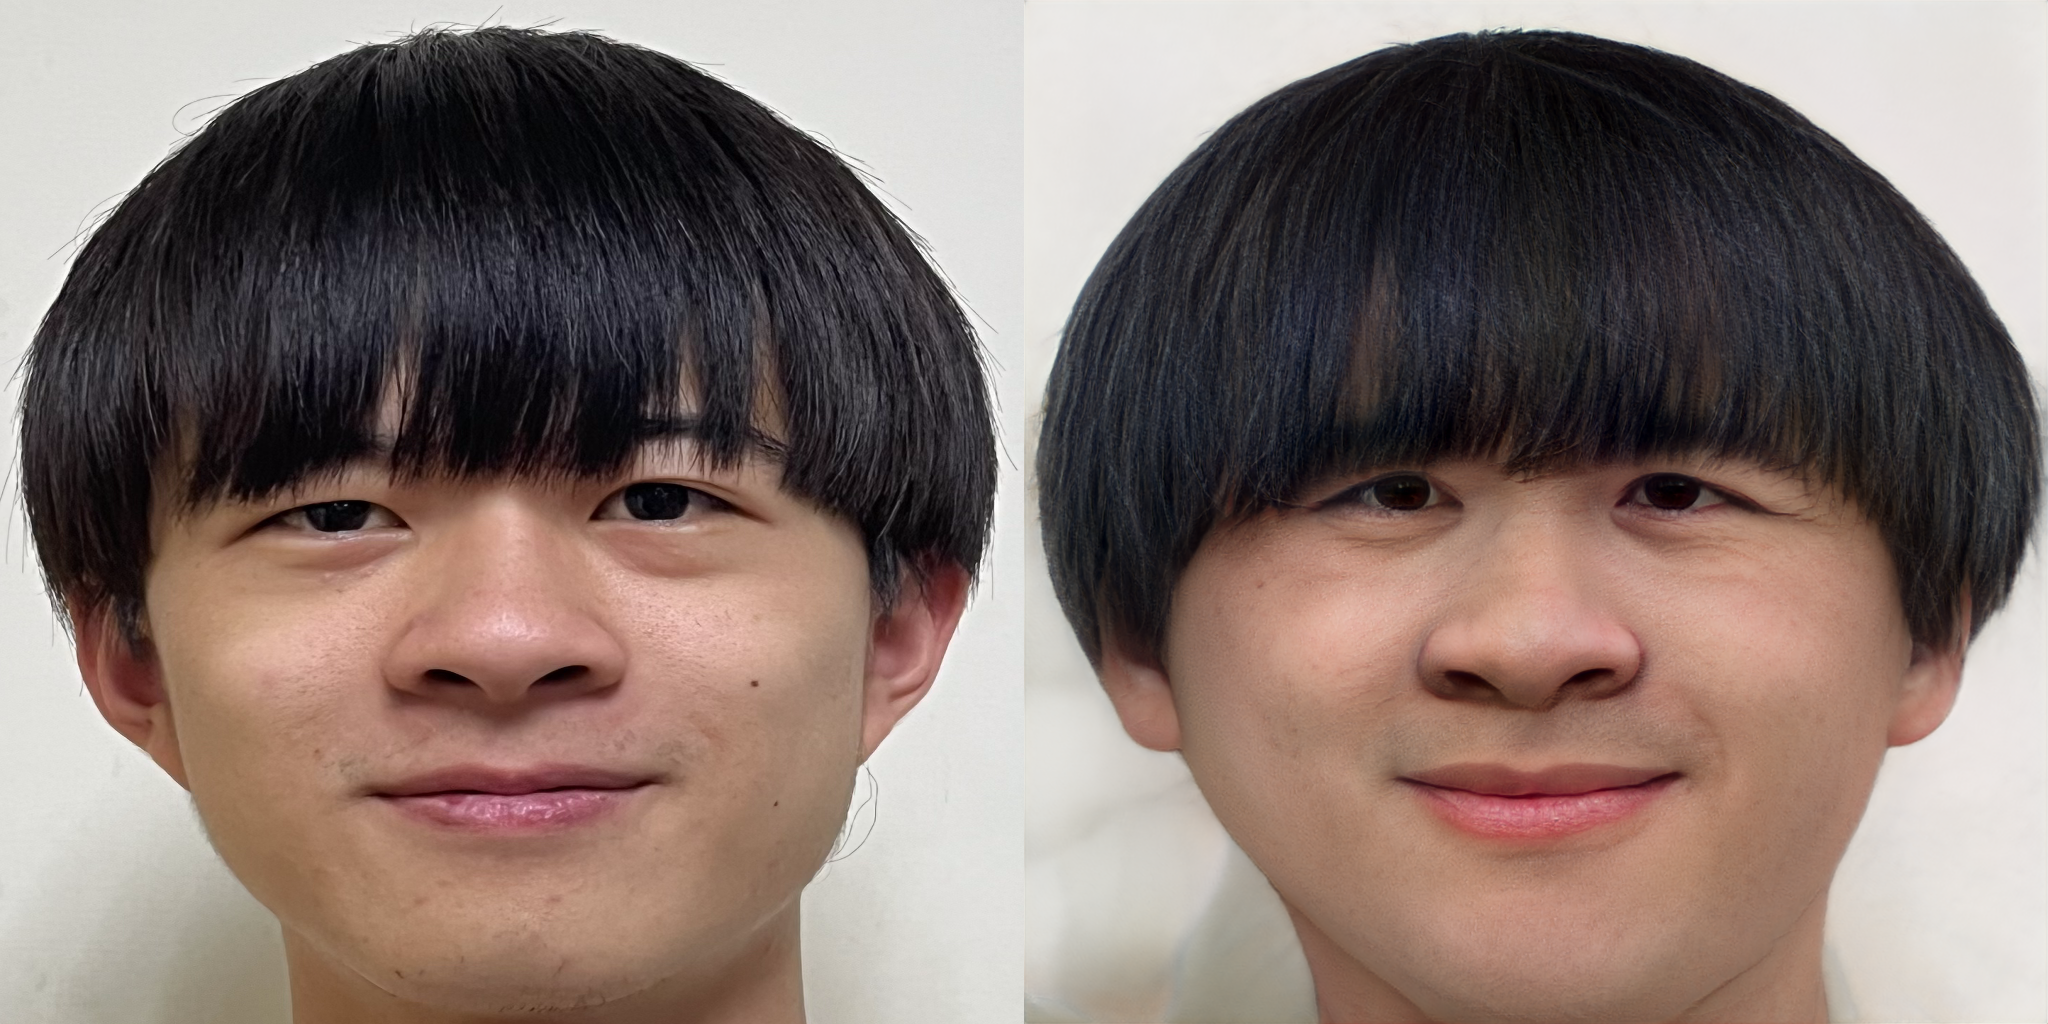
\includegraphics[scale=0.05]{fig/couple_result_cmp.png}
  \caption{face position problem}
  \label{fig:face position problem}
\end{figure}

\subsection{Human Pose Estimation}

We conduct an experiment on the accuracy of real-time human pose. The result is shown in Table \ref{table:eval}. We can see that we achieve an excellent performance in raising hand and punching, which achieves 100\% accuracy. As for the last action "hands together", the accuracy is less than other. The main reason is that when we perform this action, the key point position of our hands will get very close, leading to self-occlusion. Under such condition, we observe that the prediction result of mediapipe becomes more unstable, so the average accuracy drops to 75\%.

\begin{table}
\begin{center}
\begin{tabular}{c|c|c|c|c}
\hline
Action & Test Case & \thead{Correct (L)} & \thead{Correct (R)} & \thead{Accuracy  (\%)}\\
\hline 
raise left hand & 10 & 10 & 10 & \textbf{100}\\
% \hline
raise right hand & 10 & 10 & 10& \textbf{100}\\
% \hline
punch left & 10 & 10 & 10 & \textbf{100}\\
% \hline
punch right & 10 & 10 & 10 & \textbf{100}\\
% \hline
hands together & 10 & 8 & 7 & 75 \\
\hline
\end{tabular}
\captionof{table}{Evaluation table for pose2action conversion. \texttt{correct (L)} and \texttt{correct (R)} stands for the number of correctly detected case for left person and right person in the game interface respectively.}
\label{table:eval}
\end{center}
\end{table}
% \begin{center}
% \begin{tabular}{c|c|c|c|c}
% \hline
% Action & test case & \thead{correct (L)} & \thead{correct (R)} & \thead{Accuracy  (\%)}\\
% \hline 
% raise left hand & 10 & 10 & 10 & \textbf{100}\\
% % \hline
% raise right hand & 10 & 10 & 10& \textbf{100}\\
% % \hline
% punch left & 10 & 10 & 10 & \textbf{100}\\
% % \hline
% punch right & 10 & 10 & 10 & \textbf{100}\\
% % \hline
% hands together & 10 & 8 & 7 & 75 \\
% \hline
% \end{tabular}
% \captionof{table}{Evaluation table for pose2action conversion. \texttt{correct (L)} and \texttt{correct (R)} stands for the number of correctly detected case for left person and right person in the game interface respectively.}
% \label{table:eval}
% \end{center}